
\section{Modeling choices: Grid and time}
\label{sec:modeling-computational}

\subsection{Computational box} \label{subsect:coords}
\optsection{Computational box}
\optseealso{Grid}

PISM does all simulations in a computational box\index{PISM!computational box} which is rectangular in the PISM coordinates.  The coordinate system has horizontal coordinates $x,y$ and a vertical coordinate $z$.  The $z$ coordinate is measured positive upward from the base of the ice.  The vector of gravity is in the negative $z$ direction.  The surface $z=0$ is the base of the ice, however, and thus is usually not horizontal in the sense of being parallel to the geoid.   The surface $z=0$ is the base of the ice both when the ice is grounded and when the ice is floating.

When the ice is grounded, the true physical vertical coordinate $z'$, namely the coordinate measure relative to a reference geoid, is given by $z'=z+b(x,y)$ where $b(x,y)$ is the bed topography.  The surface $z'=h(x,y)$ is the surface of the ice.  In the grounded case the equation $h(x,y)=H(x,y)+b(x,y)$ always applies if $H(x,y)$ is the thickness of the ice.

In the floating case, the physical vertical coordinate is $z'=z-(\rho_i/\rho_s) H(x,y)$ where $\rho_i$ is the density of ice and $\rho_s$ the density of sea water.  Again $z=0$ is the base of the ice, which is the surface $z' = -(\rho_i/\rho_s) H(x,y)$.  The surface of the ice is $h(x,y) = (1-\rho_i/\rho_s) H(x,y)$.  The \emph{flotation criterion} $-(\rho_i/\rho_s) H(x,y) > b(x,y)$ applies.

The computational box can extend downward into the bedrock.  As $z=0$ is the base of the ice, the bedrock corresponds to negative $z$ values regardless of its true (i.e.~$z'$) elevation.

The extent of the computational box, along with its bedrock extension downward, is determined by four numbers \texttt{Lx}, \texttt{Ly}, \texttt{Lz}, and \texttt{Lbz} (see Figure \ref{fig:rectilinearbox} and Table \ref{tab:compbox}).  The first two of these are half-widths and have units of kilometers when set by options or displayed.

\begin{figure}[ht]
\centering
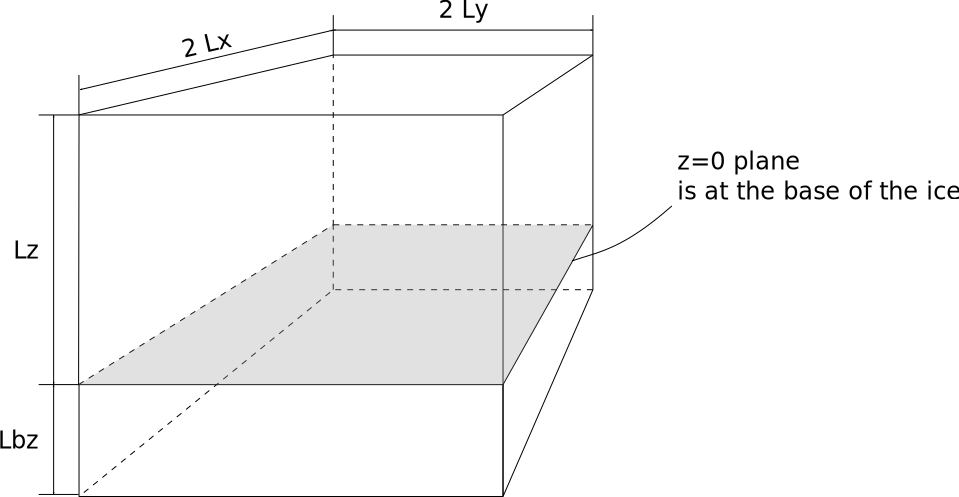
\includegraphics[width=4.0in,keepaspectratio=true]{rectilinearbox}
\caption{PISM's computational box.}
\label{fig:rectilinearbox}
\end{figure}

\begin{table}
  \centering
  \begin{tabular}{llp{0.7\linewidth}}
    \toprule
    \textbf{Option} & \textbf{Meaning}
    \\\midrule
    \txtopt{Lx}{(km)} & Half-width of the computational domain (in the $x$-direction) \\
    \txtopt{Ly}{(km)} & Half-width of the computational domain (in the $y$-direction) \\
    \txtopt{Lz}{(meters)} & Height of the computational domain; must exceed maximum ice thickness \\
    \txtopt{Lbz}{(meters)} & Depth of the computational domain in the bedrock thermal layer
    \\\bottomrule
  \end{tabular}
  \caption{Options defining the extent of PISM's computational box.}
  \label{tab:compbox}
\end{table}


\subsection{Spatial grid}
\label{subsect:grid}
\optsection{Grid!space}

The PISM grid\index{PISM!grid} covering the computational box is equally spaced in horizontal ($x$ and $y$) directions.  Vertical spacing in the ice is quadratic by default but optionally equal spacing can be chosen; choose with options \txtopt{z_spacing}{[\texttt{quadratic}, \texttt{equal}]} at bootstrapping.  The grid read from a ``\texttt{-i}'' input file is used as is.  The bedrock thermal layer model always uses equal vertical spacing.

The grid is described by four numbers, namely the number of grid points \texttt{Mx} in the $x$ direction, the number \texttt{My} in the $y$ direction, the number \texttt{Mz} in the $z$ direction within the ice, and the number \texttt{Mbz} in the $z$ direction within the bedrock thermal layer.  These are specified by options \intextoption{Mx}, \intextoption{My}, \intextoption{Mz}, and \intextoption{Mbz}, respectively. The defaults are 61, 61, 31, and 1, respectively.  Note that \texttt{Mx}, \texttt{My}, \texttt{Mz}, and \texttt{Mbz} all indicate the number of grid \emph{points} so the number of grid \emph{spaces} are one less, thus 60, 60, 30, and 0 in the default case.

The lowest grid point in a column of ice, at $z=0$, coincides with the highest grid point in the bedrock, so \texttt{Mbz} must always be at least one.  Choosing \texttt{Mbz}$>1$ is required to use the bedrock thermal model.  When a thermal bedrock layer is used, the distance \texttt{Lbz} is controlled by the \texttt{-Lbz} option.  Note that \texttt{Mbz} is unrelated to the bed deformation model (glacial isostasy model); see section \ref{subsect:beddef}.

In the quadratically-spaced case the spacing near the ice/bedrock interface is about four times finer than it would be with equal spacing for the same value of \texttt{Mz}, while the spacing near the top of the computational box is correspondingly coarser.  For a detailed description of the spacing of the grid, see the documentation on \texttt{IceGrid::compute_vertical_levels()} in the PISM class browser.

The user should specify the grid when using \texttt{-bootstrap} or when initializing a verification test (section \ref{sec:verif}) or a simplified-geometry experiment (section \ref{sec:simp}).  If one initializes PISM from a saved model state using \texttt{-i} then the input file determines all grid parameters.  For instance, the command

\begin{verbatim}
$  pismr -i foo.nc -y 100
\end{verbatim}

\noindent should work fine if \texttt{foo.nc} is a PISM output file.  Because \texttt{-i} input files take precedence over options,

\begin{verbatim}
$  pismr -i foo.nc -Mz 201 -y 100
\end{verbatim}

\noindent will give a warning that ``\texttt{PISM WARNING: ignoring command-line option '-Mz'}''.


\subsubsection{Parallel domain distribution}
\label{sec:domain-dstribution}
\optsection{Grid!domain distribution}

When running PISM in parallel with \texttt{mpiexec -n N}, the horizontal grid is distributed across $N$ processes\footnote{In most cases one process corresponds to one ``core'' of your computer.}.  PISM divides the grid into $N_x$ parts in the $x$ direction and $N_y$ parts in the $y$ direction.  By default this is done automatically, with the goal that $N_x\times N_y = N$ and $N_x$ is as close to $N_y$ as possible.  Note that $N$ should, therefore, be a composite (not prime) number.

Users seeking to override this default can specify $N_x$ and $N_y$ using the \intextoption{Nx} and \intextoption{Ny} command-line options.

Once $N_x$ and $N_y$ are computed, PISM computes sizes of sub-domains $M_{x,i}$ so that $\sum_{i=1}^{N_x}M_{x,i} = \mathrm{Mx}$ and $M_{x,i} - \left\lfloor \mathrm{Mx} / N_x \right\rfloor < 1$. To specify strip widths $M_{x,i}$ and $M_{y,i}$, use command-line options \intextoption{procs_x} and \intextoption{procs_y}. Each option takes a comma-separated list of numbers as its argument. For example,
\begin{verbatim}
$ mpiexec -n 3 pisms -Mx 101 -My 101 -Nx 1 -Ny 3 -procs_x 101 -procs_y 20,61,20
\end{verbatim}
%$ - match dollar signs to make emacs happy
splits a $101 \times 101$ grid into 3 strips along the $x$ axis.

To see the parallel domain decomposition from a completed run, see the \texttt{rank} variable in the output file, e.g.~using \texttt{-o_size big}.  The same \texttt{rank} variable is available as a spatial diagnostic field (subsection \ref{sec:saving-spat-vari}).


\subsection{Model time}
\label{sec:time}
\optsection{Grid!time}

Table \ref{tab:timeoptions} gives the command-line options which control PISM time.  If option \texttt{-ys} is absent then the start year is read from the input file (if present) or it defaults to zero.  The default value for the end year is the start year plus the given (\texttt{-y}) run length.  If both \texttt{-ys} and \texttt{-ye} are used then the run length is set to the difference.  Using all three of \texttt{-ys}, \texttt{-y} and \texttt{-ys} is not allowed; this generates an error message.

\begin{table}
\begin{tabular}{lp{0.8\linewidth}}\\
\toprule
\textbf{Option} & \textbf{Meaning}\\
\midrule
\txtopt{y}{(years)} & Number of model years to run.\\
\txtopt{ys}{(years)} & Model year at which to start the run.  Also resets the model time, ignoring any time in the input file.\\
\txtopt{ye}{(years)} & Model year at which to end the run.\\
\bottomrule
\end{tabular}
\caption{Command-line options controlling PISM time.}
\label{tab:timeoptions}
\end{table}


\subsection{Calendars}
\label{sec:calendars}
\index{Time!calendars}

Most of PISM, and its ice dynamics core in particular, only needs to know the length of the current time-step.  Internally PISM stores time in ``seconds since a specified moment'' and thus PISM generally does not use or need a calendar.\footnote{Note seconds are part of SI units.}  We refer to PISM internal time as \emph{model time}.

One can select a calendar for more precise control of the model time, however.  A ``calendar'' is a concept that is part of the \href{http://cf-pcmdi.llnl.gov/documents/cf-conventions/1.6/cf-conventions.html}{CF Metadata Conventions}.  Choosing a calendar is appropriate for runs for specific temporal periods like ``the 18th-century'' or ``1989--2010''.  The calendar is generally needed because  specific knowledge of lengths of months and years is required to use climate data properly or to facilitate model validation.

PISM uses \href{http://meteora.ucsd.edu/~pierce/calcalcs/index.html}{CalCalcs} by David~W.~Pierce to perform calendric computations.  This lets us support all the calendars \href{http://cf-pcmdi.llnl.gov/documents/cf-conventions/1.6/cf-conventions.html#calendar}{defined} by the CF Metadata Conventions document except for the \texttt{366_day} (\texttt{all_leap}) calendar.

Time units in PISM's output files always contain a reference date because it is required by the CF metadata conventions.

By default PISM does not use a calendar. This is appropriate for runs that do not require precise application of forcing data or reporting on particular dates (paleo-climate runs, for example).  In this mode PISM ignores the reference date in time unit specifications (such as ``\texttt{days since 1969-7-20}''), though the value set using \config{reference_date} configuration parameter is saved in (is passed forward into) output files.

\begin{table}
  \centering
  \begin{tabular}{lp{0.7\linewidth}}
    \texttt{gregorian} or \texttt{standard} & Mixed Gregorian/Julian calendar used today.\\
    \texttt{proleptic_gregorian} & Gregorian calendar extended to dates before 1582-10-15.\\
    \texttt{noleap} or \texttt{365_day} & Calendar with fixed-length 365-day years\\
    \texttt{360_day} & Calendar with fixed-length 360-day years divided into 30-day months\\
    \texttt{julian} & Julian calendar \\
    \texttt{none} & no calendar\\
  \end{tabular}
  \caption{Calendars supported by PISM. Please see \href{http://meteora.ucsd.edu/~pierce/calcalcs/calendars.html}{CalCalcs documentation} for details.}
  \label{tab:calendars}
\end{table}

Selecting a calendar using the \config{calendar} configuration parameter or the \intextoption{calendar} command-line option enables calendar-based time management; see Table \ref{tab:calendars}.  The implications of selecting a calendar are:
\begin{itemize}
\item PISM uses the \texttt{units} attribute of coordinate variables
  \emph{literally} (including the reference date) in unit conversions. Please
  make sure that the \variable{time} variable in all forcing files has the
  units attribute such as ``\texttt{days since 2012-1-1}''. PISM will stop with
  an error message if a time variable does not have a reference date in its
  unit specification.
\item It is important to use units that are a fixed multiple of ``seconds'',
  such as ``\texttt{minutes since 1989-1-1}'' or ``\texttt{days since
    1999-12-31}'' and avoid ``months'' and ``years''. (PISM uses UDUNITS-2 to
  convert units, and in UDUNITS one month is always interpreted as
  $\frac{1}{12}\cdot 365.242198781$ days.) Please see the 
  \href{http://cf-pcmdi.llnl.gov/documents/cf-conventions/1.6/cf-conventions.html#time-coordinate}{CF
    Conventions} document for details.
\item PISM uses dates in standard output:
\begin{verbatim}
...
   time interval (length)   [2012-01-01, 2021-12-31]  (10.000 years)
...
S 2012-05-26:  0.00011    0.6306   0.00000000           0.00000
$v$Eh m (dt=0.10000)
S 2012-07-01:  0.00014    0.6306   0.00000000           0.00000
\end{verbatim}
\end{itemize}

Just like in the no-calendar mode, run length, run start and run end
times are specified using \intextoption{y}, \intextoption{ys} and
\intextoption{ye} command-line options, respectively. Arguments of
these options are interpreted in a slightly different manner, though:
\begin{itemize}
\item the run length option \texttt{-y} takes an \emph{integer}
  argument, interpreted as the number of \emph{calendar} years
\item options \texttt{-ys} and \texttt{-ye} take \emph{dates} as arguments.
\end{itemize}

For example, either of the following commands sets up a run covering the 21$^{st}$ century:
\begin{verbatim}
$ pismr -calendar gregorian -ys 2001-1-1 -y 100 ...
$ pismr -calendar standard -ys 2001-1-1 -ye 2101-1-1 ...
\end{verbatim}
(These option combinations are equivalent.)

It is also possible to run PISM for the duration of the available forcing data using the \fileopt{time_file} option.  The command
\begin{verbatim}
$ pismr -calendar gregorian -time_file forcing.nc
\end{verbatim}
%$ - match dollar signs to make emacs happy
will extract the reference date and run length from \texttt{forcing.nc}, respecting time bounds.

When a non-trivial calendar is selected, spatial and scalar time-series can be saved daily, monthly or yearly using these calendric computations. See sections~\ref{sec:saving-time-series} and~\ref{sec:saving-spat-vari}.

\subsubsection{Re-starting an interrupted run using \texttt{-time_file}}
\label{sec:time-file-restart}

If a run using \texttt{-time_file} gets interrupted but manages to save a backup, re-starting with \texttt{-time_file} will attempt to re-do the entire run because options \texttt{-y}, \texttt{-ys}, and \texttt{-ye} are ignored:
\begin{verbatim}
# This run gets killed but leaves backup.nc:
$ pismr -i input.nc -time_file time.nc -o output.nc
# This WILL NOT start from the time saved in backup.nc
# and continue until the end time in time.nc
$ pismr -i backup.nc -time_file time.nc -o output.nc
\end{verbatim}
In this case we want to set the start time of the run from \texttt{backup.nc}, but use the end time from \texttt{time.nc}. To achieve this, use the option \intextoption{time_file_continue_run}.
\begin{verbatim}
# This run gets killed but leaves backup.nc:
$ pismr -i input.nc -time_file time.nc -o output.nc
# This WILL continue until the end time in time.nc, starting from backup.nc
$ pismr -i backup.nc -time_file time.nc -o output.nc -time_file_continue_run
\end{verbatim}

\subsection{Diagnostic computations}
\label{sec:diagnostic-computations}

A ``diagnostic'' computation can be defined as one where the internal state does not evolve.  The internal state of PISM is the set of variables read by ``\texttt{-i}''.  You can ask PISM to do a diagnostic computation by setting the run duration to a small number such as $0.001$ years (about $9$ hours). The duration to use depends on the modeling setup, but should be smaller than the maximum time-step allowed by PISM's stability criteria. Such short runs can also be used to look at additional fields corresponding to the current model state.

As an example, consider these two runs:
\begin{verbatim}
pisms -y 6000 -o foo.nc
pismr -i foo.nc -y 0.001 -o bar.nc -o_size big
\end{verbatim}

\noindent The result of the second (short) run is a NetCDF file \texttt{bar.nc} which contains the full three-dimensional velocity field in the scalar NetCDF variables \texttt{uvel}, \texttt{vvel}, and \texttt{wvel}, as well as many other variables.  The file \texttt{foo.nc} does not contain many of these fields because it was written with the default output size of \texttt{medium}.  The ``\texttt{-y 0.001}'' run has diagnostically ``filled-in'' all the fields which PISM can model at a time step, but the run duration was chosen so as to avoid significant model state evolution during the run.

This diagnostic mode is often associated to the modeling of ice shelves and ice streams.  Subsection \ref{sec:ross} describes using a short ``diagnostic'' run to model the Ross ice shelf \cite{MacAyealetal}.  Verification tests I and J, section \ref{sec:verif}, are diagnostic calculations using the SSA.

The NetCDF model state saved by PISM at the end of an \emph{evolution} run (i.e.~with ``\texttt{-y }$Y$'' for $Y>0$) does not, under the default \texttt{-o_size medium} output size, contain the three-dimensional velocity field.  Instead, it contains just a few more variables than those which are needed to restart the run with \texttt{-i}.  One can  force PISM to save all the supported diagnostic quantities at the end of a time-stepping run using the option \texttt{-o_size big}.  Or one can go back and do a ``\texttt{-y small_number}'' diagnostic run using \texttt{-o_size big}.


\subsection{Disabling PISM components}
\label{sec:turning-off}
\optsection{Disabling PISM components}

Certain major model components, unlike more peripheral ones like bed deformation or calving, are ``on'' by default.  They do not need to be turned on explicitly.  For example, the SIA computation is so common that it would be a hassle to require an option to turn it on every time you need it.

But sometimes one wants to disable particular components, during model spin-up, for example.  PISM has the following ``off'' switches:
\begin{itemize}
\item \intextoption{no_mass} disables the mass-continuity (conservation of mass) step
\item \intextoption{energy none} disables the conservation of energy computation
\item \intextoption{energy cold} makes PISM use temperature instead of enthalpy in the energy conservation code
\item \intextoption{stress_balance none} disables the stress balance computation (useful for testing surface mass balance inputs)
\end{itemize}


\subsection{Dealing with more difficult modeling choices}
\label{subsec:hard-choices}\optsection{Dealing with more difficult modeling choices}

Most uses of an ice sheet model depend on careful modeling choices in situations where there are considerable uncertainties \emph{and} the model results depend strongly on those choices.  There may be, at the present state of knowledge, \emph{no clear default values} that PISM can provide.  Furthermore, the available PISM options and sub-models are known to \emph{not} be sufficient for all users.  Thus there are modelling situations for which we know the user may have to do a great deal more hard work than just choose among PISM runtime options.

Here are example cases where users have worked hard:
\begin{itemize}
\item User made use of available data in order to choose parameters for existing PISM models.  These parameters then override PISM defaults.
\begin{center} % our UAF current situation with Greenland
\fbox{ \begin{minipage}[t]{5.0in}
\emph{Example}.  Use regional atmosphere model output to identify PDD parameters suitable for modeling surface mass balance on a particular ice sheet.  Then supply these parameters to PISM by a \texttt{-config\_override} file.
\end{minipage} }
\end{center}
\item User wrote code, including code which modified current PISM internals, either to add additional processes or to ``correct'' PISM default process models.
\begin{center} % the ocean coupler-related Potsdam marine ice sheet mods
\fbox{ \begin{minipage}[t]{5.0in}
\emph{Example}.  Add a new sub-ice-shelf melt model by modifying C++ code in the \texttt{src/coupler/} directory.
\end{minipage} }
\end{center}
\item User simplified the model in use, instead of the default which was more elaborate.
\begin{center} % Nick's -yield_stress constant choice
\fbox{ \begin{minipage}[t]{5.0in}
\emph{Example}.  Instead of using the PISM default mechanism connecting basal melt rate and basal strength, bypass this mechanism by generating a map of yield stress \texttt{tauc} directly and supplying it as input.
\end{minipage} }
\end{center}
\end{itemize}


%%% Local Variables: 
%%% mode: latex
%%% TeX-master: "manual"
%%% End: 

% LocalWords:  
